\renewcommand*\chapterpagestyle{scrheadings}
\chapter{Introduction and System Overview}

This project is a frontend designed mainly to run on a Raspberry Pi with dedicated hardware, but other Linux/Unix-like systems are supported too. It is an extension to a voice assistant diploma thesis, focusing on providing a user-friendly interface to record audio from the user and forward it to the backend for processing.

\section{Project Scope}
The project scope is as follows:
\begin{itemize}
    \item Efficient communication with the backend, with the goal of limiting response delays to 1 second.
    \item Playing back responses from the backend, where the user has the option to receive the output either as text or as audio.
    \item Allowing the user to choose between text input, push-to-talk, and voice activation modes.
\end{itemize}

\section{Background and Motivation}
Voice assistants have steadily gained popularity in recent years, yet they are often perceived as minor enhancements rather than essential tools. This project aims to change that perception by providing a voice assistant frontend solution that can enhance users' workflows without being intrusive --- doing what other voice assistants are known to do but also offering more significant quality-of-life improvements like workspace management and speech-to-text input.

\section{Technical Challenges}
The development of this project is expected to encounter several technical challenges, including but not limited to:
\begin{itemize}
    \item \textbf{Voice Activation:} Implementing an effective voice activation system necessitates continuous listening capabilities. This can be achieved either through a wake-word detection mechanism or an advanced language model that can discern commands from regular speech. Both approaches require careful consideration of computational efficiency and responsiveness.
    \item \textbf{Security:} The ability to execute arbitrary commands poses a significant security risk. It is imperative to implement strict access controls and validation mechanisms to prevent unauthorized actions and protect the user from potential threats posed by malicious actors.
    \item \textbf{User Experience:} Ensuring a seamless and intuitive user experience is vital for the adoption of the voice assistant. This includes minimizing response times, providing clear feedback, and designing an accessible and user-friendly interface.
    \item \textbf{Low Latency:} Ensuring efficient communication with the backend is essential to achieve the goal of response delays no longer than 1 second on a Raspberry Pi. While most of the heavy lifting is done by the backend, communication protocols still need to be optimized to ensure low latency.
\end{itemize}

\section{Choice of Framework}
Several front-end frameworks were taken into consideration when deciding what to use for the project. These include:
\begin{itemize}
    \item Vue.js
    \item Godot
    \item Qt
    \item SDL
    \item Embedded Graphics
\end{itemize}

Initially, \texttt{Vue.js} and \texttt{Godot} were considered due to prior experience with these frameworks. However, given that the voice assistant frontend would run on a Raspberry Pi where performance is crucial for ensuring a smooth user experience, these options were ruled out. While low-level frameworks like \texttt{SDL} and \texttt{Embedded Graphics} were available, their steep learning curve and limited industry adoption made them impractical choices. Ultimately, \texttt{Qt} was selected for its robust performance, extensive industry usage, comprehensive documentation, and the fact that its the framework that is used by my desktop environment (KDE Plasma), so it would have seamless integration with my personal system.

\section{System Architecture}
The complete voice assistant consists of two parallel projects: this Qt-based frontend and a Rust backend being developed as an ongoing diploma thesis. The frontend serves as the user interface layer, providing efficient access to the backend's voice processing capabilities.

\begin{figure}[H]
    \centering
    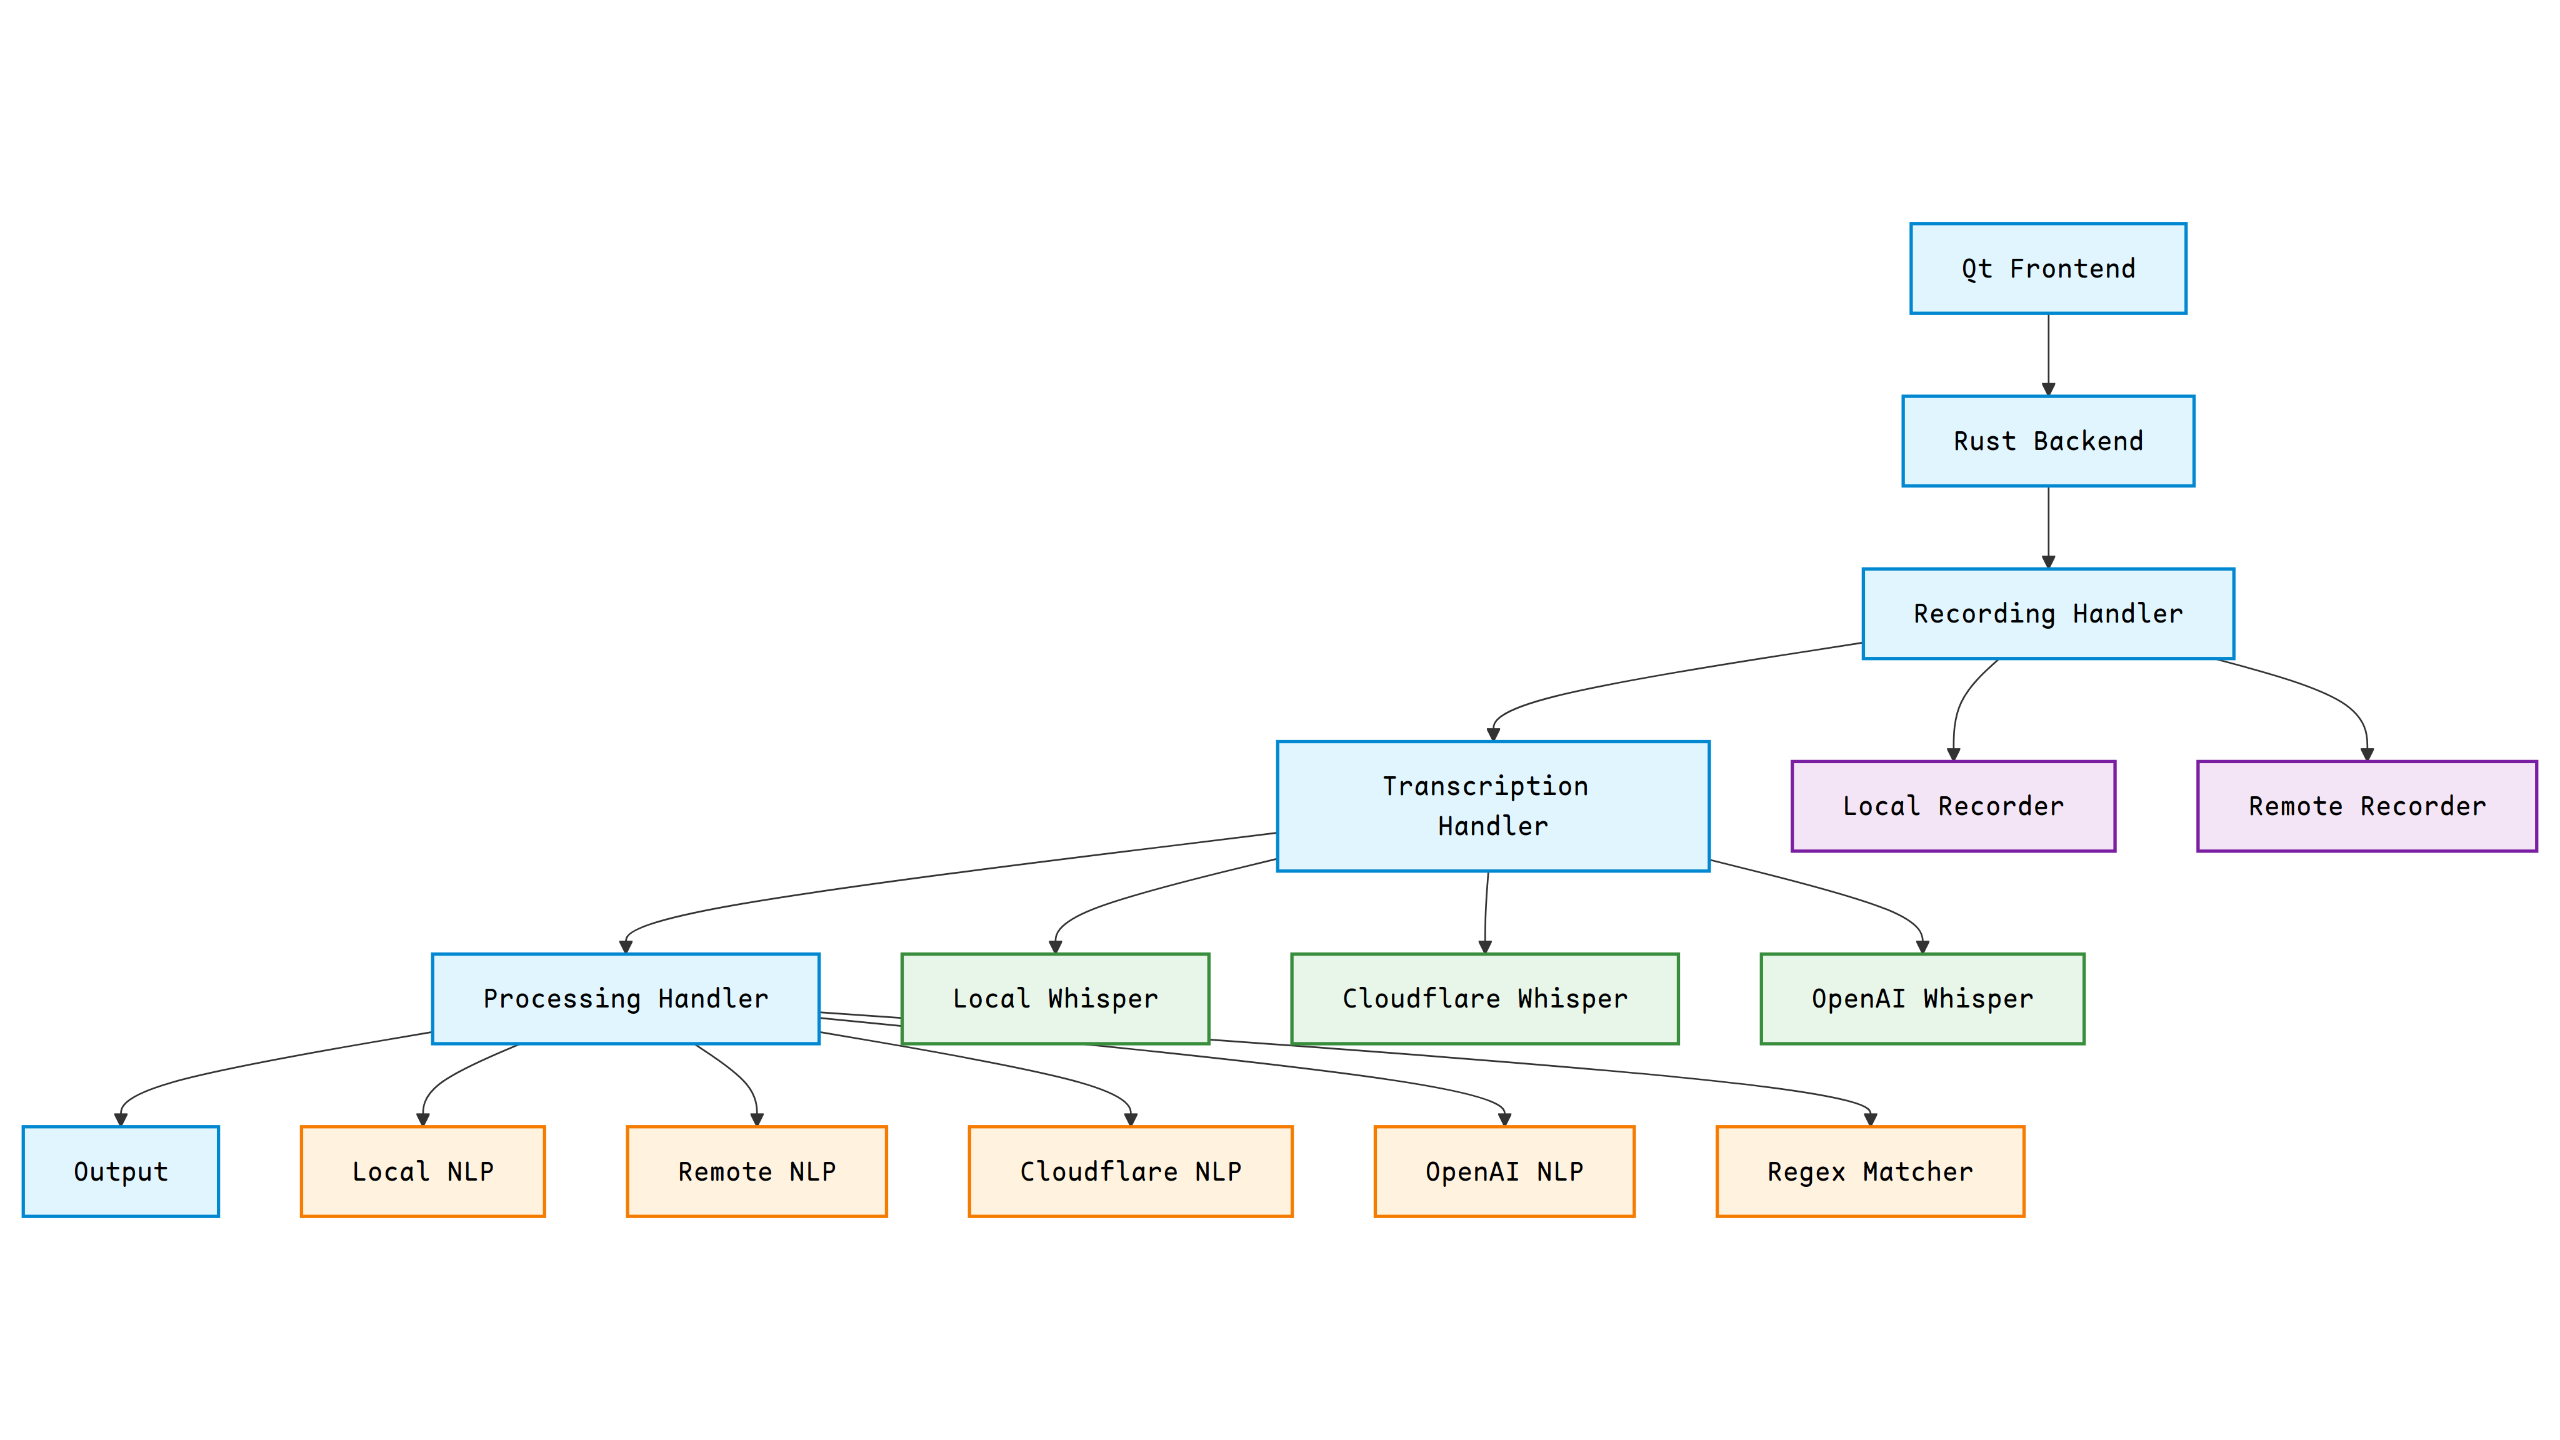
\includegraphics[width=\textwidth]{assets/stackchart}
    \caption{System architecture showing the Qt frontend (current project scope) and the Rust backend components (parallel diploma thesis). The processing pipeline flows from the frontend through various backend stages, each offering multiple implementation options.}
    \label{fig:system-architecture}
\end{figure}

\subsection{Frontend}
The Qt-based frontend layer handles:
\begin{itemize}
    \item User interface and interaction
    \item Audio recording control
    \item Communication with backend
    \item Result presentation
\end{itemize}

\subsection{Backend}
The backend system, currently under development, comprises several processing stages:
\begin{itemize}
    \item \textbf{Recording Stage:} Implements both local and remote recording capabilities:
    \begin{itemize}
        \item Local Recorder for direct hardware access
        \item Remote Recorder for distributed setups
    \end{itemize}
    \item \textbf{Transcription Stage:} Provides multiple transcription options:
    \begin{itemize}
        \item Local Whisper for offline processing
        \item Cloudflare Whisper for edge computing
        \item OpenAI Whisper for cloud-based processing
    \end{itemize}
    \item \textbf{Processing Stage:} Implements various NLP options:
    \begin{itemize}
        \item Local NLP for offline processing
        \item Remote NLP for distributed processing
        \item Cloudflare NLP for edge computing
        \item OpenAI NLP for advanced language models
        \item Regex Matcher for simple pattern matching
    \end{itemize}
    \item \textbf{Output Stage:} Handles the final processing results
\end{itemize}

The modular architecture enables flexible deployment configurations. Users can choose between local processing for privacy-conscious applications or cloud-based processing for enhanced capabilities, with the frontend adapting seamlessly to either choice.

\section{Communication}
The communication between frontend and backend components is implemented through TCP sockets, providing reliable data transfer while maintaining low latency required for real-time voice processing.

\subsection{Socket Architecture}
The backend establishes a local TCP socket bound to port 8080, acting as a server for incoming client connections. Current implementation is limited to single-client operation, though work is underway to implement asynchronous client handling.

The communication protocol implements a simple command-response pattern, where the frontend sends commands and receives either processing results or error messages. Two primary commands are supported:
\begin{itemize}
    \item \texttt{START\_RECORDING}: Initiates audio capture
    \item \texttt{STOP\_RECORDING}: Terminates capture and processes the audio
\end{itemize}

\subsection{Implementation}
The backend command handler demonstrates the core logic:

\begin{minted}{rust}
let response = match line.trim() {
    "START_RECORDING" => {
        self.recorder.start()?;
        recording_active = true;
        "Recording started.".to_string()
    }
    "STOP_RECORDING" if recording_active => {
        let audio = self.recorder.stop()?;
        recording_active = false;
        self.transcriber.transcribe(&audio).await?
    }
    "STOP_RECORDING" => "No recording in progress.".to_string(),
    _ => "Unknown command.".to_string(),
};

writeln!(writer, "{}", response)?;
\end{minted}

The implementation maintains recording state and provides error handling for both recording and transcription operations. Response messages are transmitted back to the frontend for user feedback or error display.

\subsection{Future Development}
Several improvements are planned for the communication subsystem:
\begin{itemize}
    \item Asynchronous client handling
    \item Extended command set
    \item Enhanced error recovery mechanisms
\end{itemize}

\section{Qt Framework}
The Qt framework is a comprehensive toolkit designed for creating cross-platform applications with a focus on performance and user experience. It is particularly well-suited for projects that require a responsive and visually appealing interface, such as the voice assistant frontend described in this documentation. This section provides an overview of the key components and concepts of the Qt framework, including qmake, signals and slots, Qt Creator, and .ui files.

\subsection{qmake}
qmake is the build system tool used by Qt to manage the compilation and linking of applications. It simplifies the build process by automatically generating Makefiles based on project files (.pro). A typical .pro file includes information about the source files, headers, and other resources needed for the project. Here is an example of a simple .pro file:

\begin{verbatim}
TEMPLATE = app
TARGET = myapp
QT += core gui
\end{verbatim}

The .pro file specifies that the project is an application (TEMPLATE = app), the target executable is named "myapp", and it uses the Qt core and GUI modules. Additional elements like source files, headers, and forms can be specified in similar fashion.

\subsection{Signals and Slots}
One of the most powerful features of Qt is its signals and slots mechanism, which facilitates communication between objects. Signals are emitted when a particular event occurs, and slots are functions that respond to these signals. This mechanism allows for a flexible and decoupled design.

The following example demonstrates connecting a button's click signal to a label's text update slot:

\begin{verbatim}
connect(button, &QPushButton::clicked, label, &QLabel::setText);
\end{verbatim}

In this example, the QPushButton's clicked signal is connected to the QLabel's setText slot. When the button is clicked, the label's text is updated accordingly.

\subsection{Qt Creator and .ui Files}
Qt Creator is an integrated development environment specifically designed for Qt development. It provides comprehensive tools for code editing, debugging, and UI design. The integrated UI editor allows developers to create and arrange widgets using a visual interface, generating .ui files that represent the UI layout in XML format.

These .ui files can be integrated into applications using the uic (User Interface Compiler) tool, which converts the .ui files into C++ code during the build process. This generated code creates and configures the UI elements exactly as designed in Qt Creator's visual editor.

\subsection{Layouts and Widgets}
Qt provides a wide range of widgets for building user interfaces, including buttons, labels, text fields, and more. These widgets can be arranged using layout managers, which ensure that the UI elements are positioned and resized correctly.

The framework includes several types of layout managers: QHBoxLayout, QVBoxLayout, QGridLayout, and QFormLayout. Each layout manager arranges widgets in a specific way. QHBoxLayout arranges widgets horizontally, while QVBoxLayout arranges them vertically.
